\section{\acs{hl7} \& \acs{fhir}} \label{sec:hl7fhir}

Wichtig um die Interoperabilität in Gesundheitswesen zu gewährleisten, sind syntaktische \ac{it}-Standards wie \ac{fhir}, der neueste Standard von \ac{hl7} mit Fokus auf den aktuellen Web-Standards und einer einfachen Implementierung \cite{telemedizin, hl7, fhir}.

\subsection{\acs{hl7}} \label{subsec:hl7}

\acf{hl7} ist eine nicht gewinnorientierte, \ac{ansi}-akkreditierte Standardisierungsorganisation zur Bereitstellung eines umfassenden Frameworks und dessen Standards auf der 7. Ebene (Anwendungsschicht) im \ac{iso}/\ac{osi} Modell  
%(\ref{sec:isoosi})
, für den Austausch, die Integration, das Teilen und den Abruf elektronischer Gesundheitsinformationen \cite{telemedizin, ehealtOk, hl7}. \ac{hl7}-Schnittstellen unterstützen die Kommunikation von Softwaresystemen in klinischen Einrichtungen und somit das Management, die Erbringung und Bewertung von Gesundheitsdiensten \cite{ehealtOk, hl7, fhir}.

\subsection{\acs{fhir}} \label{subsec:fhir}

Der \acf{fhir}-Standard eignet sich für den Einsatz in verschiedenen Szenarien, wie den Datenaustausch auf nationaler und internationaler Ebene, in einem regionalen Netzwerk, zwischen Systemen innerhalb einer Organisation und den Datenaustausch mit mobilen Applikationen \cite{ehealtOk, fhir}. 

\ac{fhir} besteht aus drei Bausteinen: Ressourcen (Resources), Referenzen (References) und Profile (Profiles) \cite{fhir}.

In \ac{fhir} werden Konzepte aus der realen Welt als Ressourcen mit entsprechenden für Menschen und Maschinen lesbaren Werten dargestellt \cite{ehealtOk}. Diese wiederum sind logische Einheiten des Datenaustausches mit einem konkreten, definierten Verhalten und eindeutiger Semantik \cite{fhir}. Die Definition der Ressourcen deckt häufig die meisten Anwendungsfälle \cite{ehealtOk}. Jede Ressource besteht aus strukturierten Daten, Narrativen und Ergänzungen (Extensions) \cite{fhir}. Während die strukturierten Daten 80\% der weitverbreiteten Einsatzszenarien abdecken, lassen sich manche Ressourcen durch die Ergänzungen erweitern, die nicht in \ac{fhir} erhältlich sind, um speziellere Anwendungsfälle abdecken zu können \cite{fhir, ehealtOk}. Die Narrative sind dann menschenlesbare Texte, um den Inhalt der Ressourcen zusammenzufassen \cite{fhir}.

Die Referenzen ermöglichen es, dass mehrere Ressourcen und deren Informationseinheiten aufeinander verweisen können, um Beziehungen aufzubauen \cite{fhir}. Ein Beispiel davon sind die \glqq Observation\grqq{}-Ressourcen mit den Werten der Messungen im Erweiterungsmodul \glqq Intensivmedizin\grqq{} verweisen auf die \glqq Patient\grqq{}-Ressourcen mit der Information der behandelnden Personen in dem Basismodul \glqq Person\grqq{} des Kerndatensatzes der \ac{mii} (\ref{fig:mii}).

Viele Werte in den \ac{fhir}-Ressourcen sind optional, sodass eine Umsetzung kompatibel ist, wenn sie nur die minimal obligatorischen Daten liefert. Diese Werte können von außen über die Profile modifiziert werden, und können wiederum sich aufeinander verweisen \cite{ehealtOk}. Das bedeutet die \ac{fhir}-Profile sind die Spezifikationen, die die \ac{fhir}-Ressourcen beschreiben und definieren, z. B. die Festlegung von konkreten Codesystemen \cite{fhir, fhircompact}.

\begin{comment}
Der \ac{fhir}-Standard besitzt fünf Begriffe für die Beschreibung der Stabilität-Ebene \cite{fhircompact}:

\begin{enumerate}
	\item Draft: Dies beschreibt eine nicht komplette oder nicht ausreichende überprüfende Spezifikation. Die Nutzung der Spezifikationen unter dieser Ebene ist riskant.
	\item Trial Use: Solche Spezifikationen sind noch nicht veröffentlicht, trotzdem gut überprüft und von den Autoren für die Nutzung in Systemen empfohlen.
	\item Normative: Diese sind die stabilen veröffentlichten Spezifikationen.
	\item Informative: Diese Spezifikationen definieren keine Regeln und sind für die Assistenz der Implementierung konzipiert.
	\item Deprecated: Die Spezifikationen unter dieser Ebene sind veraltet, und beinhalten Orientierungshilfe für die Anwender und Anwenderinnen. Somit sollen sie verhindern, neue Features in diesen Spezifikationen einzufügen.
\end{enumerate}
\end{comment}

Ein zuvor genannter Aspekt von \ac{fhir} ist seine Fokussierung auf moderne Webprotokolle. Somit können die \ac{fhir}-Ressourcen, die auf einem Server liegen, über eine Schnittstelle via \ac{http} abgefragt werden \cite{telemedizin, ehealtOk}. Außerdem ist das Datenformat für diese Übertragung auch von \ac{fhir} festgelegt, diese kann entweder \ac{xml} oder \ac{json} sein \cite{ehealtOk}. Diese zwei Formate sind weitverbreitet und besitzen eine hohe Akzeptanz durch ihre Versatilität \cite{fhirformat}.

Die \ac{fhir}-Profile können auf verschiedene Art und Weise dargestellt werden. Die am häufigsten benutzten Arten der Darstellung sind logische Tabellen, \ac{xml}- und \ac{json}-Schemata \cite{fhirformat}.

\subsubsection{Logische Tabelle} \label{subsubsec:logtab}

Eine logische Tabelle eines \ac{fhir}-Profils beinhaltet die Spalten: Name, Flags, Card., Type und Description \& Constraints, wobei diese letzte Spalte beim Anklicken eines Elements eingeblendet wird \cite{fhirformat}. \ref{fig:logic-table} zeigt ein Teil der logischen Tabelle eines \ac{fhir}-Profils des Erweiterungsmoduls \glqq Intensivmedizin\grqq{}.

\begin{figure}[ht]
	\centering
	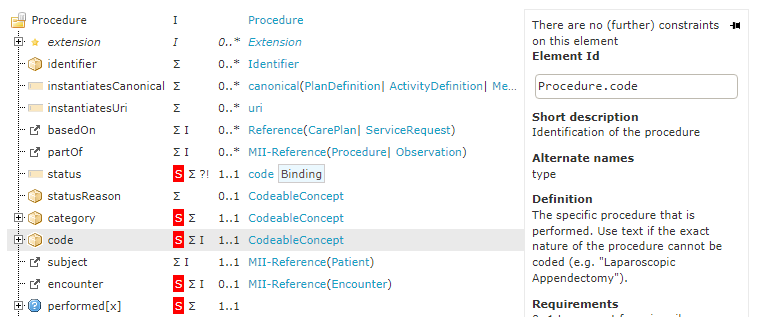
\includegraphics[height=6cm]{figures/beatmung}
	\caption[Logische Tabelle eines \acs{fhir}-Profils]{Fragment der logischen Tabelle des \acs{fhir}-Profils Beatmung des Erweiterungsmoduls \glqq Intensivmedizin\grqq{} des Kerndatensatzes der \acs{mii}.}
	\label{fig:logic-table}
\end{figure}

\begin{itemize}
	\item Name: Name eines Elements in der \ac{fhir}-Ressource. Das Icon bezeichnet den Inhalt des Elements. In der \ref{fig:icons} wird die Bedeutung der Icons erklärt.
	\item Flags: Entscheidende Informationen darüber, wie das Element implementiert werden sollte.
	\begin{itemize}
		\item S: Dieses Element muss unterstützt werden.
		\item I: Elemente mit diesem Symbol definieren Randbedingungen oder sind Teile davon, z. B. das Element \texttt{code} definiert die benutzten Codesysteme bei der \glqq Procedure\grqq{}-Profile (\ref{fig:logic-table})
		\item $\sum$: Diese Elemente sind Teile einer Ressource.
		\item ?!: Das sind modifizierende Elemente, z. B. das Element \texttt{status} beschreibt den Zustand einer \glqq Procedure\grqq{}-Ressource, nämlich \texttt{final}, wenn die Ressource in einer Endversion sich befindet (\ref{fig:logic-table}).
	\end{itemize}
	\item Card.: Cardinality - untere und obere Grenze, wie häufig dieses Element in der Ressource erscheinen darf.
	\item Type: Typ des Elements. Hier erscheint auch der Link zur Definition des Typs.
	\item Description \& Constraints: Beschreibung des Elements und Details über die Einschränkungen.
\end{itemize}

\begin{figure}[ht]
	\centering
	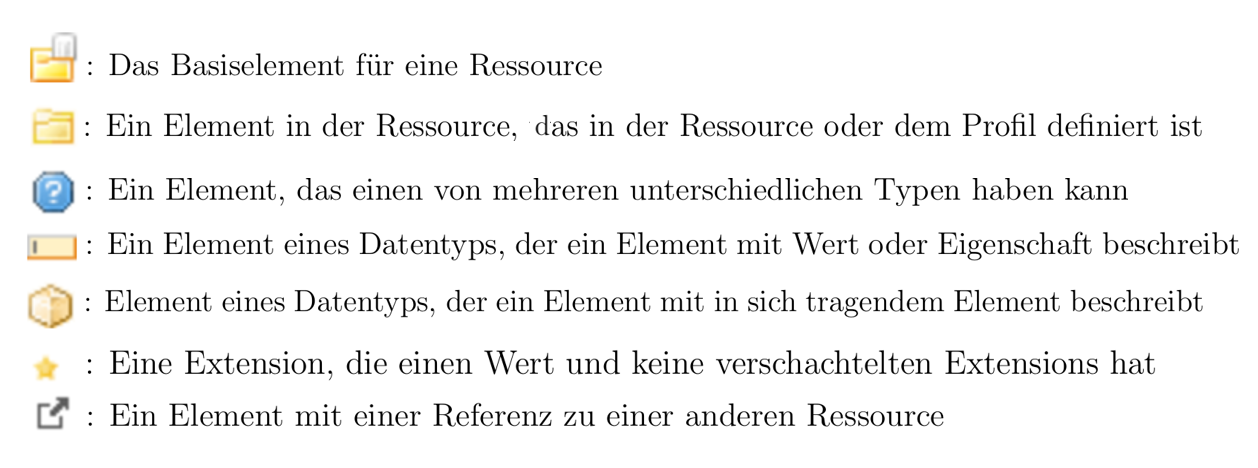
\includegraphics[height=5cm]{figures/icons_description}
	\caption[Beschreibung der meist benutzten \acs{fhir}-Icons]{Beschreibung der meist benutzten \acs{fhir}-Icons.}
	\label{fig:icons}
\end{figure}


\subsubsection{\acs{xml}} \label{subsubsec:xml}

Die Metasprache \acf{xml} hat ihre Wurzeln im Internet und wurde vom \ac{w3c} im Jahr 1998 veröffentlicht und dessen aktuelle Fassung ist die fünfte von 2008 \cite{grundinfo}. Als Metasprache können mit Hilfe von \ac{xml} andere anwendungsspezifische Sprachen, wie \ac{fhir}, definiert werden. Mit \ac{xml} können auch Daten gespeichert oder übertragen werden \cite{interop, grundinfo}.

Ein \ac{xml}-Dokument ist für das Computer-Processing konzipiert, trotzdem kann dieses Dokument von Menschen gelesen werden, denn Dokumente im \ac{xml}-Format sind zur selben Zeit Text-Dateien \cite{grundinfo}. Die Regeln bei \ac{xml}-Dateien sind strikt, sodass Fehler in den Anwendungen verhindert werden. Alle \ac{xml}-Dokumente beinhalten verbundene Knoten in einer Baumstruktur, wo alle Knoten von einer einzelnen Wurzel stammen, das so genannte Element \cite{interop}. Für die Auszeichnung von Elementen werden Tags \glqq $<$, $>$, $/$$>$ \grqq{} verwendet \cite{grundinfo}. Attribute werden in \ac{xml} benutzt, um die Information der Elemente einzufügen \cite{interop, quality}. Der Code \ref{list:xmlpatient} zeigt die \ac{fhir}-\ac{xml}-Datei für die Definition einer Person.

\begin{lstlisting}[caption={[Beispiel einer \acs{fhir}-Ressource in XML] Beispiel einer \acs{fhir}-Ressource für eine Person in XML.},language=xml, label=list:xmlpatient, captionpos=b]
	<?xml version="1.0" encoding="UTF-8"?> 
	
	<Patient xmlns="http://hl7.org/fhir">
	  <id value="xds"/> 
	  <text> 
	    <status value="generated"/>
	  </text> 
	  <identifier> 
	    <use value="usual"/> 
 	    <type> 
	      <coding> 
	        <system value="http://terminology.hl7.org/CodeSystem/v2-0203"/> 
	        <code value="MR"/> 
	      </coding> 
	    </type> 
	    <system value="urn:oid:1.2.3.4.5"/> 
	    <value value="89765a87b"/> 
	  </identifier> 
	  <active value="true"/> 
	  <gender value="male"/> 
	  <birthDate value="1989-05-27"/> 
	  <address> 
	    <postalCode value="55122"/> 
	  </address> 
	  <managingOrganization> 
	    <reference value="Organization/2"/> 
	  </managingOrganization> 
	</Patient>
\end{lstlisting}

Die grundlegende analytische und Design-Aufgabe der Nutzung von \ac{xml} ist die Erstellung von Schemata \cite{grundinfo}. Die Struktur eines \ac{xml}-Dokuments wird in einem Schema beschrieben, das wiederum in \ac{xml} geschrieben ist. Das Schema bestimmt die Struktur eines Dokumenttyps, die für alle Dokumente dieser Art gleich ist \cite{interop, grundinfo}. Es legt die Tags und die Verbindungen zwischen den Elementen fest. Die Schemata werden anhand eines oder mehrerer Schemata mit Hilfe von Anwendungen validiert \cite{grundinfo}. In \ac{hl7} sind zwei Schemasprachen häufig verbreitet, die \ac{xsd} (\ac{xml}-Schemata) des \ac{w3c} zur Strukturdefinition von \ac{xml}-Dokumenten, und Schematron zur Validierung von Inhalt und Struktur von \ac{xml}-Doku- menten \cite{interop}. \ac{xml}-Schemata werden normalerweise als separate Datei mit der Erweiterung .xsd erstellt und über eine Namespace-Deklaration mit der Datei verlinkt \cite{interop}.

\subsubsection{\acs{json}} \label{subsubsec:json}

\acf{json} ist ein, auf Features der Skriptsprache JavaScript basiertes, menschlesbares Datenaustauschformat für die Übertra- gung der Information zwischen Anwendungen \cite{jsondef}. Aus diesem Grund kann die Sprache selbst die Daten in \ac{json}-Format decodieren, und die Daten können als native JavaScript-Objekte direkt angewendet werden \cite{interop}. 

Dadurch dass \ac{json} einfacher als \ac{xml} ist und viele Programmiersprachen schon \ac{json}-Bibliotheken implementiert haben, ist \ac{json} das bevorzugte Datenaustauschformat zwischen Anwendungen im unterschiedlichen Kontext, z. B. \ac{fhir}-Server und Webanwendungen, und damit eine geeignete Option, um Interoperabilität in Gesundheitswesen zu gewährleisten \cite{interop, jsondef}. Der Code \ref{list:jsonpatient} zeigt die \ac{fhir}-\ac{json}-Datei für die Definition einer Person.

\begin{lstlisting}[caption={[Beispiel einer \acs{fhir}-Ressource in JSON] Beispiel einer \acs{fhir}-Ressource für eine Person in JSON.},language=JavaScript, label=list:jsonpatient, captionpos=b]
{
  "resourceType": "Patient",
  "id": "xds",
  "text": 
  {
    "status": "generated",
   },
  "identifier": 
  [
    {
      "use": "usual",
	  "type": {
	  "coding": 
	  [
	    {
	      "system": "http://terminology.hl7.org/CodeSystem/v2-0203",
	      "code": "MR"
	    }
	  ]
	},
	  "system": "urn:oid:1.2.3.4.5",
	  "value": "89765a87b"
	}
  ],
  "active": true,
  "gender": "male",
  "birthDate": "1989-05-27",
  "address": 
  [
    {	  
	  "postalCode": "55122",
	}
  ],
  "managingOrganization": 
  {
    "reference": "Organization/2"
  }
}
\end{lstlisting}

\ac{json} besteht aus sechs Datentypen für die Darstellung von Entitäten der realen Welt \cite{jsondef}:
\begin{enumerate}
	\item String: Unicode-Zeichen
	\item Number: Gleitkomma-Format von JavaScript mit doppelter Genauigkeit
	\item Boolean: Die Werte \texttt{true} und \texttt{false} ohne Anführungszeichen
	\item Null: Leerer Wert
	\item Object: Gruppe von Namens- oder Wertpaaren zwischen $\{$ $\}$
	\item Array: Geordnete Sammlung von Werten
\end{enumerate}
